\documentclass[conference]{IEEEtran}
\IEEEoverridecommandlockouts
\usepackage{graphicx,amsmath,amssymb,booktabs,array,url,xcolor}
\usepackage[hidelinks]{hyperref}
\usepackage{textcomp}
\graphicspath{{figs/}}
\renewcommand{\arraystretch}{1.15}

\begin{document}

\title{Disciplined Specification Search and Model-Class Evaluation for\\ Macroeconomic VAR Forecasting: A Leakage-Free Study on US Quarterly Data}

\author{\IEEEauthorblockN{Nicholas Hong}
\IEEEauthorblockA{Nanyang Technological University\\ Email: nhong001@e.ntu.edu.sg}%
\thanks{This work is for educational and research purposes and does not constitute investment advice. All data are drawn from public sources. All figures and tables derive from a single seeded script (seed 20260710); code and data-construction scripts are available on request.}}

\maketitle

\begin{abstract}
We present a reproducible, leakage-free framework for selecting and evaluating classical vector autoregression (VAR) forecasting models on US quarterly macroeconomic data, and apply it to establish a set of honest null results. A theory-pruned block forward selection, guarded by hard validity filters for stability, residual whiteness, parsimony, and conditioning, selects a parsimonious oil-augmented core VAR over a real-activity, price, policy-rate, and exchange-rate core. We show that the filters catch overfitting that raw out-of-sample root mean squared error (RMSE) rewards: a household net worth block lowers relative RMSE yet fails the parsimony and whiteness gates. Extending the comparison across estimator classes, ordinary least squares (OLS), Minnesota Bayesian VAR, and ridge, LASSO, and elastic-net VAR, including wide-information shrinkage variants, no model is distinguishable from a univariate autoregression by the Model Confidence Set at these sample sizes. We further quantify two pitfalls in common applied practice. Full-sample Hodrick-Prescott filtering of the policy rate introduces look-ahead bias whose endpoint revision reaches sixty-six percent of the cyclical component's own standard deviation, and year-over-year overlapping transforms inject moving-average residual autocorrelation that causes every specification to fail the whiteness test. The message is that disciplined parsimony and leakage-free evaluation dominate methodological sophistication in short macroeconomic samples.
\end{abstract}

\begin{IEEEkeywords}
Vector autoregression, forecast evaluation, Model Confidence Set, Bayesian VAR, shrinkage estimation, Hodrick-Prescott filter, look-ahead bias, macroeconomic forecasting.
\end{IEEEkeywords}

\section{Introduction}
Applied macroeconomic forecasting with vector autoregressions confronts a persistent tension. The information set is large, the sample is short, and the analyst is free to search over variable sets, transformations, lag structures, and estimators. Unconstrained search invites data snooping, while overly rigid modeling discards useful structure. This paper builds a framework that navigates that tension explicitly, and reports what a defensible search actually finds on US data.

Our contribution is threefold. First, we formalize a block-level forward selection that searches over economically motivated groups of variables rather than the power set of individual series, and pair it with hard validity filters so that a specification is eligible only if it is stable, has approximately white residuals, and respects a degrees-of-freedom budget. Second, we conduct a fair model-class comparison on a single winning specification, holding sample, split, horizon, and metric fixed, and summarize it with the Model Confidence Set (MCS) of Hansen, Lunde, and Nason \cite{hln2011}. Third, we quantify two construction choices that are common in practice but damaging in a forecasting context: full-sample Hodrick-Prescott (HP) filtering \cite{hp1997} and year-over-year (YoY) overlapping transforms.

The results are deliberately unglamorous. The disciplined baseline is a four-variable core plus oil as an exogenous regressor. Its measurable edge over a random walk is confined to the real exchange rate and, at longer horizons, output. No estimator, Bayesian or regularized, beats a simple autoregression by a statistically distinguishable margin. We argue that reporting such nulls, rather than tuning them away, is the correct scientific posture for this class of problem.

\section{Data and Transformations}
All series are US quarterly observations obtained from the Federal Reserve Economic Data (FRED) public interface and, for utilization-adjusted total factor productivity, from the Federal Reserve Bank of San Francisco \cite{fernald2014}. Table~\ref{tab:data} lists the variables and their stationarity transforms. Flow and price series enter as annualized quarterly log changes, $400\,\Delta \ln x_t$; oil enters as $100\,\Delta \ln x_t$; the policy rate enters in levels; and utilization-adjusted TFP is already a growth rate. A robustness section replaces the core flow transforms with YoY percent changes to match a common reporting convention.

\begin{table}[t]
\caption{Variables and stationarity transforms}
\label{tab:data}
\centering
\small
\begin{tabular}{@{}lll@{}}
\toprule
Role & Series (FRED id) & Transform \\
\midrule
Core: output & Real GDP (GDPC1) & $400\,\Delta\ln$ \\
Core: prices & Core PCE price (PCEPILFE) & $400\,\Delta\ln$ \\
Core: policy & Fed funds rate (FEDFUNDS) & level \\
Core: FX & Real broad USD, BIS (RBUSBIS) & $400\,\Delta\ln$ \\
Investment & Real GPDI (GPDIC1) & $400\,\Delta\ln$ \\
Consumption & Real PCE (PCECC96) & $400\,\Delta\ln$ \\
Oil & WTI spot (WTISPLC) & $100\,\Delta\ln$ \\
Fiscal & Real govt C+I (GCEC1) & $400\,\Delta\ln$ \\
Exports & Real exports G\&S (EXPGSC1) & $400\,\Delta\ln$ \\
Wealth & Household net worth (TNWBSHNO) & $400\,\Delta\ln$ \\
Housing & FHFA house price (USSTHPI) & $400\,\Delta\ln$ \\
Productivity & Fernald util.-adj. TFP & level (rate) \\
\bottomrule
\end{tabular}
\end{table}

The common sample is 1994Q2 to 2026Q1, or 128 quarters, with the start bound by the real broad dollar index. YoY variants begin in 1995Q1 and span 125 quarters. A Johansen trace test on the core levels returns rank zero at the five percent level, so we model stationary transforms rather than a vector error correction system.

\section{Methodology}

\subsection{Out-of-sample design and relative RMSE}
We use an expanding window with the first forecast origin at fifty-five percent of the sample. At each origin we estimate every model on data up to that origin only and forecast $h\in\{1,4\}$ quarters ahead, iterating the VAR for multistep paths. For a target $y$ we report the relative RMSE,
\begin{equation}
\mathrm{relRMSE}(y,h) = \frac{\mathrm{RMSE}_{\text{model}}(y,h)}{\mathrm{RMSE}_{\text{RW}}(y,h)},
\end{equation}
against a no-change random walk (RW), and we also compute a univariate AR benchmark whose lag order is chosen by the Bayesian information criterion (BIC). Targets on different scales are never averaged in raw RMSE; cross-model ranking uses the average rank of relative RMSE across targets. Exogenous regressors are projected forward for multistep evaluation by their own AR(BIC), so no future value enters a forecast.

\subsection{Block forward selection}
We fix a core of output, inflation, the policy rate, and the exchange rate. Candidate shock variables are grouped into economic blocks, and one representative per block is carried forward to avoid within-group collinearity. Selection is greedy at the block level: starting from the core, we add the block that most improves the mean relative RMSE at $h=1$, and stop when no block improves it. This yields on the order of ten estimable specifications rather than the power set. A variable that is plausibly exogenous for forecasting, such as oil, is tested as an exogenous regressor rather than as an additional endogenous equation.

\subsection{Validity filters}
A specification is eligible for selection only if it passes four hard filters: stability, defined as all companion eigenvalues inside the unit circle; residual whiteness, a portmanteau test with $p>0.01$; parsimony, a ratio of effective observations to parameters of at least three; and conditioning of the regressor moment matrix. These filters are applied to the full-sample fit and gate the final ranking. Their role is to prevent raw out-of-sample RMSE from rewarding specifications that overfit or violate the model assumptions.

\subsection{Significance and the Model Confidence Set}
Pairwise accuracy is assessed by the Diebold-Mariano test \cite{dm1995} for non-nested comparisons and the Clark-West test \cite{cw2007} for nested ones, since a smaller model is nested in a same-variable Bayesian VAR and in the zero-penalty limit of the shrinkage estimators. To guard against selection across many models, we compute the Model Confidence Set \cite{hln2011}, which returns the set of models that are not statistically separable from the best at a given confidence level. This is the formal answer to the data-snooping concern: a winner that sits inside a wide confidence set is reported as such.

\section{Baseline Specification Search}
Block forward selection from the core selects oil as an exogenous regressor and stops. The resulting specification, denoted CORE+OIL(x), attains a mean relative RMSE of $0.97$ at $h=1$ and $0.88$ at $h=4$. Per target at $h=1$, it records $0.84$ for output, $1.07$ for inflation, $1.13$ for the policy rate, and $0.83$ for the exchange rate. Clark-West tests against the random walk are significant for the exchange rate ($p<0.001$) and the policy rate ($p=0.013$), marginal for output ($p=0.081$), and insignificant for inflation ($p=0.176$).

The validity filters do consequential work. When the candidate set is widened to eight blocks, unconstrained forward selection prefers to add a household net worth block, which lowers the mean relative RMSE to $0.95$ and, with oil, to $0.91$, the best raw score in the run. That specification fails the parsimony filter, with an observation-to-parameter ratio of $2.3$, and in its three-block form with oil, at a ratio of $2.1$, it also fails residual whiteness at $p=0.04$. It is therefore rejected. Utilization-adjusted TFP as an exogenous regressor is admissible and has clean residuals, but its relative RMSE of $1.06$ is worse than the bare core, so it is eligible yet never selected. Table~\ref{tab:baseline} summarizes the outcome, and Fig.~\ref{fig:baseline} shows the relative RMSE surface across specifications and targets. The disciplined winner remains CORE+OIL(x). The Model Confidence Set at ninety percent places this winner in the same set as the univariate AR and the bare core for every target, and excludes the random walk only for the exchange rate.

\begin{table}[t]
\caption{Baseline specification search, $h=1$ (relRMSE vs.\ RW)}
\label{tab:baseline}
\centering
\small
\begin{tabular}{@{}lccccc@{}}
\toprule
Specification & mean & $T/k$ & stable & white & pass \\
\midrule
CORE                 & 1.04 & 3.5 & yes & yes & yes \\
CORE+OIL(x) \textit{(sel.)} & 0.97 & 3.2 & yes & yes & \textbf{yes} \\
CORE+TFP(x)          & 1.06 & 3.2 & yes & yes & yes \\
CORE+WEALTH          & 0.95 & 2.3 & yes & yes & no \\
CORE+WEALTH+OIL(x)   & 0.91 & 2.1 & yes & no ($0.04$) & no \\
\bottomrule
\end{tabular}
\end{table}

\begin{figure}[t]
\centering
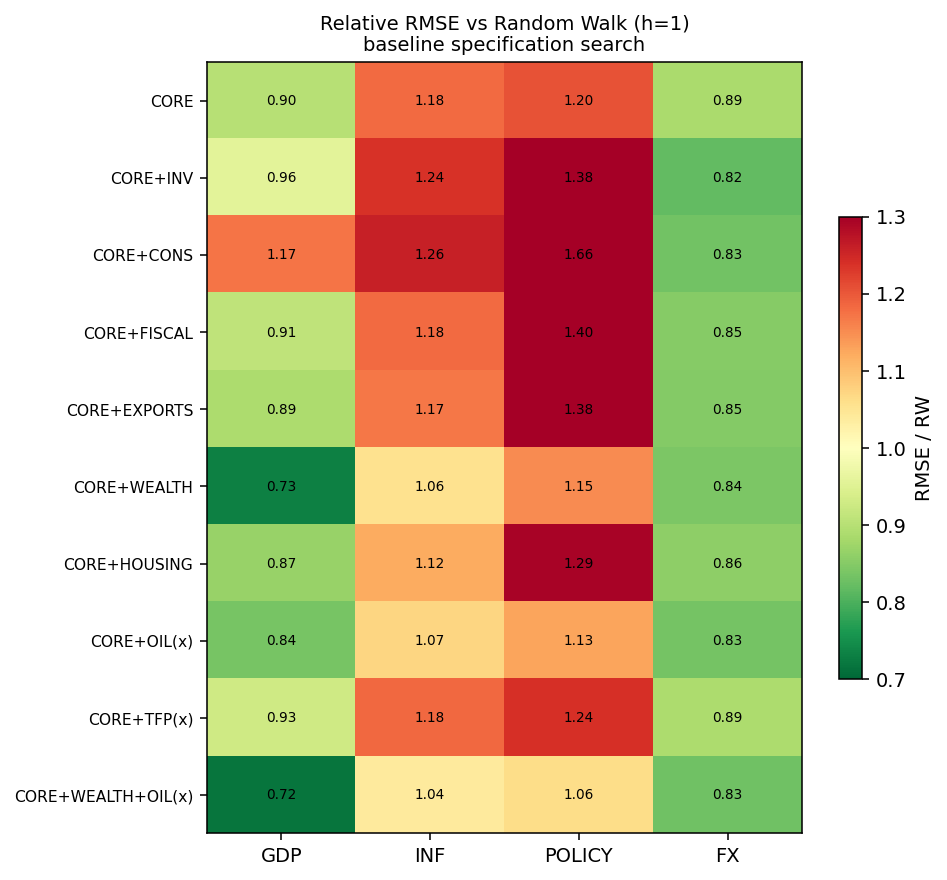
\includegraphics[width=\columnwidth]{fig_baseline.png}
\caption{Relative RMSE versus a random walk at $h=1$ across specifications (rows) and targets (columns). Values below one, in green, beat the random walk. The oil-augmented core beats the benchmark on output and the exchange rate; endogenous block additions raise the ratio and fail the validity filters.}
\label{fig:baseline}
\end{figure}

\section{Rate Representation and the HP Look-Ahead Problem}
The policy rate is borderline non-stationary, which motivates a cyclical, stance-based representation. A common choice is the deviation of the rate from an HP trend. The HP filter is two-sided, however, so a trend computed on the full sample uses future data to set the value at each date. In a recursive out-of-sample exercise this leaks information into the recent quarters on which forecasts most depend.

We quantify the effect on the fed funds rate by comparing a full-sample two-sided HP cycle with a real-time one-sided cycle, the latter defined as the last value of an expanding HP filter anchored on the rate history from 1954. The two series correlate at only $0.52$. The mean absolute revision is $0.86$ percentage points, and over the final eight quarters the mean absolute revision is $0.71$ percentage points, which is sixty-six percent of the cyclical component's own standard deviation. Fig.~\ref{fig:hp} shows the divergence and the endpoint revision, together with the Hamilton regression filter \cite{hamilton2018} as a one-sided alternative. This is consistent with the real-time output-gap unreliability documented by Orphanides and van Norden \cite{ovn2002}.

\begin{figure*}[t]
\centering
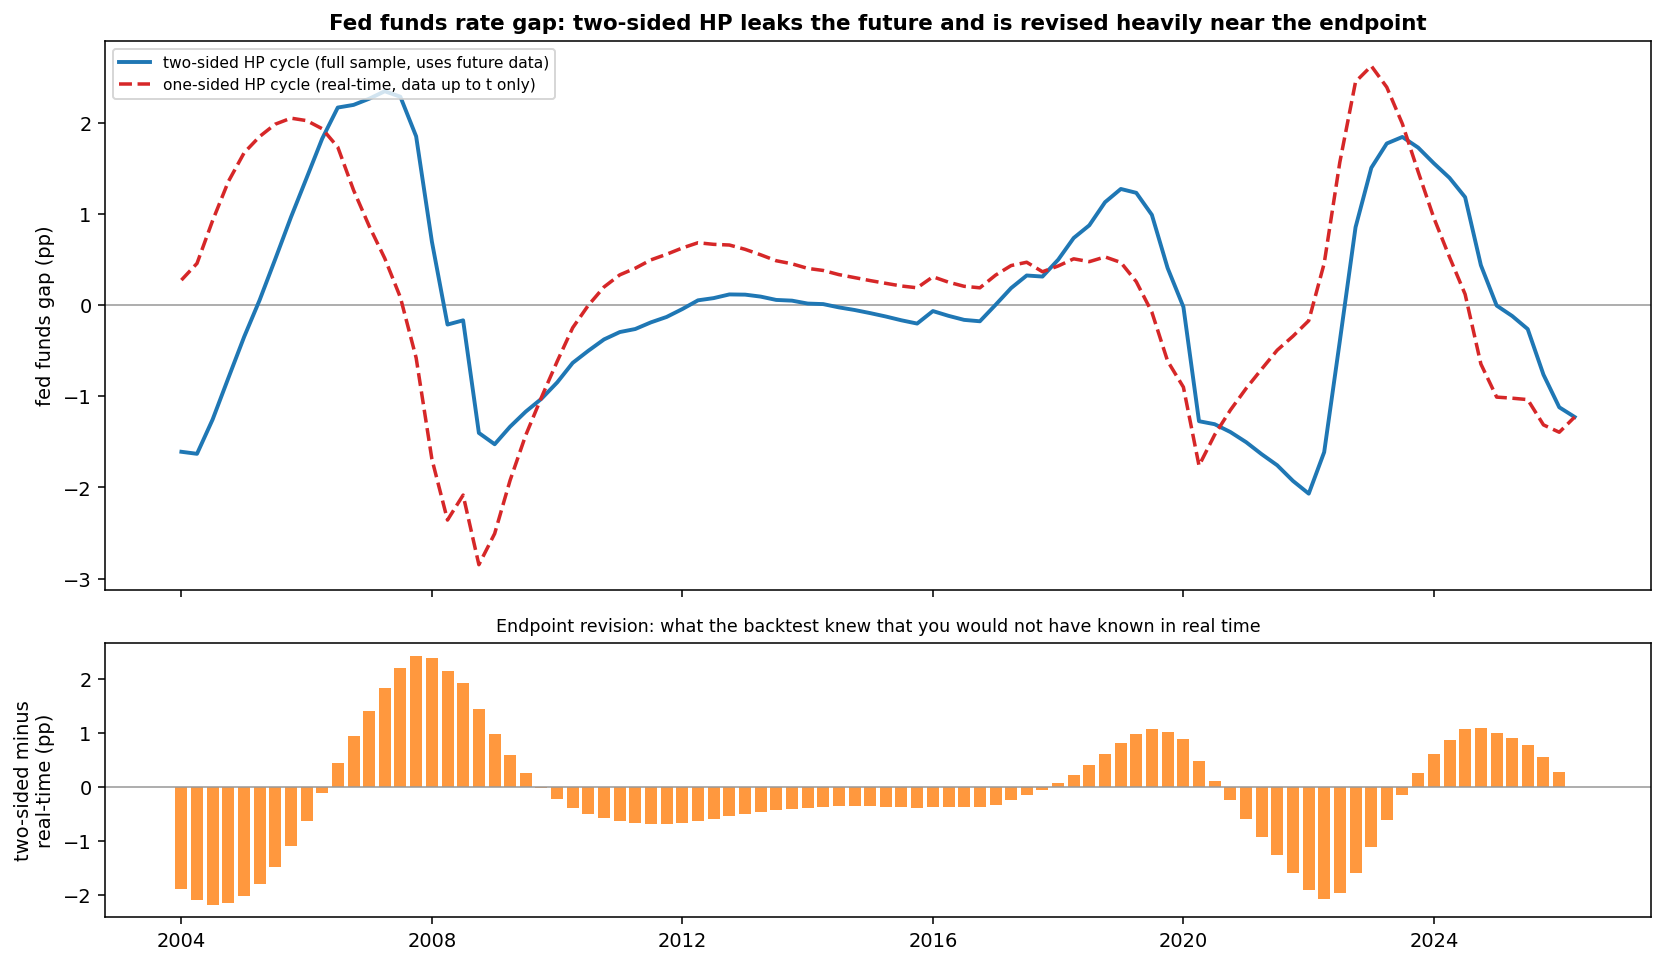
\includegraphics[width=\textwidth]{fig_hp.png}
\caption{Fed funds rate gap. Top: the full-sample two-sided HP cycle diverges from the real-time one-sided cycle and from the Hamilton filter, most visibly near the sample end. Bottom: the endpoint revision, the difference between what a full-sample backtest encodes and what was knowable in real time.}
\label{fig:hp}
\end{figure*}

We then test the rate as a level against a leakage-free one-sided gap inside the same block search, ranking on the three targets that are identical across the two representations. The two cores are close, with mean relative RMSE of $0.915$ for the level and $0.927$ for the gap at $h=1$, the level marginally ahead. The gap improves only the rate's own forecast, at $0.75$ of the random walk against $1.13$ for the level, and these figures are on different scales and so are not directly comparable. The Model Confidence Set does not separate the two. We conclude that a rate gap is defensible for structural work but earns no forecasting advantage on the broader targets, and that it must be constructed one-sided within each training window.

\section{Model-Class Comparison}
We fix the winning specification and vary the estimator. On the small information set of CORE+OIL(x) we compare OLS, Minnesota Bayesian VAR at tight and loose settings, and ridge, LASSO, and elastic-net VAR. The Minnesota prior is implemented by dummy observations \cite{bgr2010}, so the point forecast is the posterior mean, and we verified that the tight-to-loose limit recovers OLS to machine precision. Shrinkage penalties are chosen by blocked time-series cross-validation inside each training window. We add a wide information set of ten endogenous variables plus two exogenous regressors, on which OLS is deliberately overparameterized, to test whether shrinkage plus more data can beat the parsimonious baseline. The lag order is fixed at two for every class.

Table~\ref{tab:phase2} and Fig.~\ref{fig:phase2} report the outcome. The univariate AR is the single best forecaster on average at $h=1$, with a mean relative RMSE of $0.85$. The small-system estimators cluster just behind, between $0.88$ and $0.90$. Every wide-information model is worse, and the overparameterized OLS is worst. The tight Bayesian VAR delivers the best single output forecast, at $0.69$, which is the Minnesota prior trading accuracy across targets for accuracy on output. The decisive result is the joint Model Confidence Set: at ninety percent, the set contains every estimator and the AR benchmark on all four targets, and the random walk on every target except the exchange rate. At this sample size the data cannot separate the models, so the added complexity buys nothing that can be demonstrated. The failure of the wide set also vindicates the Phase-1 filters, since the variables that could not be held by OLS carry little incremental quarterly signal for these targets.

\begin{table}[t]
\caption{Model-class comparison, mean relRMSE vs.\ RW}
\label{tab:phase2}
\centering
\small
\begin{tabular}{@{}llccc@{}}
\toprule
Model & set & $h{=}1$ & $h{=}4$ & in MCS \\
\midrule
AR(BIC)            & --    & 0.85 & 0.83 & yes \\
Ridge              & small & 0.88 & 0.88 & yes \\
BVAR-Loose         & small & 0.88 & 0.89 & yes \\
OLS                & small & 0.89 & 0.90 & yes \\
BVAR-Tight         & small & 0.89 & 0.88 & yes \\
Elastic-net        & small & 0.90 & 0.90 & yes \\
LASSO              & small & 0.90 & 0.90 & yes \\
BVAR-Tight         & wide  & 0.93 & 0.88 & yes \\
Ridge              & wide  & 0.96 & 0.93 & yes \\
Random walk        & --    & 1.00 & 1.00 & all but FX \\
LASSO              & wide  & 1.01 & 1.12 & yes \\
Elastic-net        & wide  & 1.02 & 0.99 & yes \\
OLS (overfit)      & wide  & 1.05 & 1.15 & yes \\
\bottomrule
\end{tabular}
\end{table}

\begin{figure}[t]
\centering
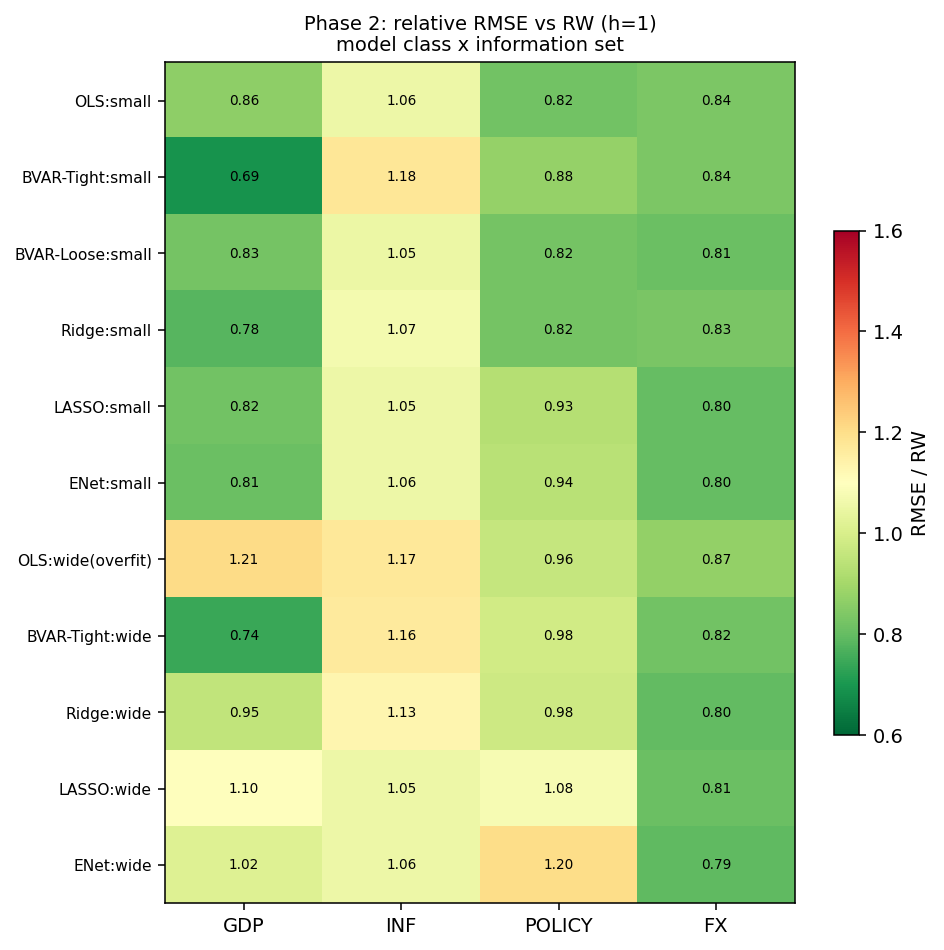
\includegraphics[width=\columnwidth]{fig_phase2.png}
\caption{Relative RMSE versus a random walk at $h=1$ by estimator (rows) and target (columns). Small-system estimators cluster near the univariate benchmark; wide-information shrinkage does not improve on the parsimonious baseline.}
\label{fig:phase2}
\end{figure}

\section{Transformation Robustness}
Reporting conventions often express macro variables as YoY percent changes. We replace the core flow transforms with YoY and re-run the search. Two effects appear. First, predictability migrates in horizon. A YoY change is a four-quarter overlapping difference, so consecutive observations share three of four quarterly innovations and the series barely moves at $h=1$, where a no-change forecast is nearly unbeatable. Output therefore loses to the random walk at $h=1$ and beats it at $h=4$, as shown in Table~\ref{tab:yoy}, the predictability having migrated to the longer horizon. Inflation, which is close to a unit root under YoY with an augmented Dickey-Fuller $p$ of $0.81$, loses at both horizons. The exchange rate beats the random walk at both horizons and by the wider margin at $h=4$. The policy rate, kept in levels, shows the reverse pattern, winning at $h=1$ and losing at $h=4$, as expected for a persistent level that mean-reverts unpredictably over a year.

Second, and more consequential, the overlapping transform injects a moving-average structure of order three into the residuals, which a short-lag VAR cannot whiten. With all core flows in YoY, every specification fails the residual-whiteness filter. This is a concrete argument against selecting lags by ordinary $t$-statistics on YoY VARs, since the standard errors are computed under an assumption the transform violates by construction, and post-selection inference is in any case invalid.

\begin{table}[t]
\caption{Transformation robustness, relRMSE vs.\ RW (CORE)}
\label{tab:yoy}
\centering
\small
\begin{tabular}{@{}lcccc@{}}
\toprule
 & \multicolumn{2}{c}{annualized q} & \multicolumn{2}{c}{year-over-year} \\
\cmidrule(lr){2-3}\cmidrule(lr){4-5}
Target & $h{=}1$ & $h{=}4$ & $h{=}1$ & $h{=}4$ \\
\midrule
Output    & 0.90 & 0.72 & 1.04 & 0.82 \\
Inflation & 1.18 & 1.08 & 1.11 & 1.15 \\
Policy (level) & 1.20 & 1.13 & 0.84 & 1.18 \\
FX        & 0.89 & 0.80 & 0.86 & 0.70 \\
\bottomrule
\end{tabular}
\end{table}

\section{Discussion}
The study supports a few practical positions. Search should be constrained by economics, at the level of blocks, and gated by validity filters that raw RMSE ignores; the net worth example shows a filter overruling a better raw score for a good reason. Estimator sophistication has a real but small and, at these samples, statistically undetectable payoff, so the honest deliverable is a confidence set rather than a single champion. Constructed regressors demand care: a two-sided filter used on the full sample leaks the future, and an overlapping transform manufactures serial correlation. Both pitfalls are quantified here rather than assumed. None of this argues against Bayesian or shrinkage methods in general, where larger cross-sections or hierarchical structure make their advantages material; it argues that on a short national quarterly panel the parsimonious baseline is hard to beat and easy to fool oneself about.

\section{Conclusion}
On US quarterly data, a disciplined and leakage-free VAR pipeline selects a four-variable core with oil as an exogenous regressor, and its genuine forecasting edge over a random walk is confined to the real exchange rate and, at a one-year horizon, output. Across OLS, Bayesian, and regularized estimators, and across narrow and wide information sets, no model is statistically separable from a univariate autoregression by the Model Confidence Set. Full-sample HP filtering and year-over-year transforms are shown to introduce look-ahead bias and residual autocorrelation, respectively. The value of the exercise is not a winning model but a transparent framework and a set of reported nulls that quantify how little the added sophistication buys at this sample size.

\begin{thebibliography}{99}
\small
\bibitem{sims1980} C.~A. Sims, ``Macroeconomics and reality,'' \emph{Econometrica}, vol.~48, no.~1, pp.~1--48, 1980.
\bibitem{litterman1986} R.~B. Litterman, ``Forecasting with Bayesian vector autoregressions,'' \emph{J. Bus. Econ. Stat.}, vol.~4, no.~1, pp.~25--38, 1986.
\bibitem{dls1984} T.~Doan, R.~Litterman, and C.~Sims, ``Forecasting and conditional projection using realistic prior distributions,'' \emph{Econometric Rev.}, vol.~3, no.~1, pp.~1--100, 1984.
\bibitem{bgr2010} M.~Ba\'nbura, D.~Giannone, and L.~Reichlin, ``Large Bayesian vector auto regressions,'' \emph{J. Appl. Econometrics}, vol.~25, no.~1, pp.~71--92, 2010.
\bibitem{glp2015} D.~Giannone, M.~Lenza, and G.~Primiceri, ``Prior selection for vector autoregressions,'' \emph{Rev. Econ. Stat.}, vol.~97, no.~2, pp.~436--451, 2015.
\bibitem{koop2013} G.~Koop, ``Forecasting with medium and large Bayesian VARs,'' \emph{J. Appl. Econometrics}, vol.~28, no.~2, pp.~177--203, 2013.
\bibitem{dm1995} F.~X. Diebold and R.~S. Mariano, ``Comparing predictive accuracy,'' \emph{J. Bus. Econ. Stat.}, vol.~13, no.~3, pp.~253--263, 1995.
\bibitem{cw2007} T.~E. Clark and K.~D. West, ``Approximately normal tests for equal predictive accuracy in nested models,'' \emph{J. Econometrics}, vol.~138, no.~1, pp.~291--311, 2007.
\bibitem{hln2011} P.~R. Hansen, A.~Lunde, and J.~M. Nason, ``The model confidence set,'' \emph{Econometrica}, vol.~79, no.~2, pp.~453--497, 2011.
\bibitem{white2000} H.~White, ``A reality check for data snooping,'' \emph{Econometrica}, vol.~68, no.~5, pp.~1097--1126, 2000.
\bibitem{hansen2005} P.~R. Hansen, ``A test for superior predictive ability,'' \emph{J. Bus. Econ. Stat.}, vol.~23, no.~4, pp.~365--380, 2005.
\bibitem{hp1997} R.~J. Hodrick and E.~C. Prescott, ``Postwar U.S. business cycles: an empirical investigation,'' \emph{J. Money Credit Bank.}, vol.~29, no.~1, pp.~1--16, 1997.
\bibitem{hamilton2018} J.~D. Hamilton, ``Why you should never use the Hodrick-Prescott filter,'' \emph{Rev. Econ. Stat.}, vol.~100, no.~5, pp.~831--843, 2018.
\bibitem{ovn2002} A.~Orphanides and S.~van Norden, ``The unreliability of output-gap estimates in real time,'' \emph{Rev. Econ. Stat.}, vol.~84, no.~4, pp.~569--583, 2002.
\bibitem{mr1983} R.~A. Meese and K.~Rogoff, ``Empirical exchange rate models of the seventies,'' \emph{J. Int. Econ.}, vol.~14, no.~1--2, pp.~3--24, 1983.
\bibitem{sw2018} J.~H. Stock and M.~W. Watson, ``Identification and estimation of dynamic causal effects in macroeconomics using external instruments,'' \emph{Econ. J.}, vol.~128, no.~610, pp.~917--948, 2018.
\bibitem{kilian2009} L.~Kilian, ``Not all oil price shocks are alike,'' \emph{Amer. Econ. Rev.}, vol.~99, no.~3, pp.~1053--1069, 2009.
\bibitem{fernald2014} J.~Fernald, ``A quarterly, utilization-adjusted series on total factor productivity,'' Federal Reserve Bank of San Francisco, Working Paper 2012-19, 2014.
\bibitem{tibshirani1996} R.~Tibshirani, ``Regression shrinkage and selection via the lasso,'' \emph{J. R. Stat. Soc. B}, vol.~58, no.~1, pp.~267--288, 1996.
\bibitem{zou2005} H.~Zou and T.~Hastie, ``Regularization and variable selection via the elastic net,'' \emph{J. R. Stat. Soc. B}, vol.~67, no.~2, pp.~301--320, 2005.
\bibitem{johansen1988} S.~Johansen, ``Statistical analysis of cointegration vectors,'' \emph{J. Econ. Dyn. Control}, vol.~12, no.~2--3, pp.~231--254, 1988.
\bibitem{pt1992} M.~H. Pesaran and A.~Timmermann, ``A simple nonparametric test of predictive performance,'' \emph{J. Bus. Econ. Stat.}, vol.~10, no.~4, pp.~461--465, 1992.
\end{thebibliography}

\end{document}
